\documentclass[12pt,twoside]{article}

\usepackage{hyperref}
\usepackage{amsmath}
\usepackage{amsfonts}
\usepackage{amssymb}
\usepackage{amsthm}
%\usepackage{palatino,lettrine}
\usepackage{fancyhdr}
\usepackage{epsfig}
\usepackage[round,comma,sort]{natbib}
\usepackage{simplemargins}
\usepackage{setspace}
\usepackage{supertabular}
\usepackage{graphicx}
\usepackage{booktabs}
\usepackage[margin=1.5cm]{caption}



\newcommand{\profs}{Prof. Jeffrey Varner}
\newcommand{\subj}{1120}

\newlength{\toppush}
\setlength{\toppush}{2\headheight}
\addtolength{\toppush}{\headsep}

\newcommand{\htitle}[3]{\noindent\vspace*{-\toppush}\newline\parbox{6.5in}
{\textit{Introduction to Chemical Engineering: ENGRI 1120}\hfill\newline
Chemical and Biomolecular Engineering, Cornell University \hfill #3\newline
%\profs\hfill Handout #1\vspace*{-.5ex}\newline
\mbox{}\hrulefill\mbox{}}\vspace*{1ex}\mbox{}\newline
\begin{center}{\Large\bf #2}\end{center}}

\newcommand{\handout}[3]{\thispagestyle{empty}
 \markboth{ENGRI 1120 #2}{ENGRI 1120 #2}
 \pagestyle{myheadings}\htitle{#1}{#2}{#3}}

%\setlength{\oddsidemargin}{0pt}
%\setlength{\evensidemargin}{0pt}
%\setlength{\textwidth}{6.5in}
%\setlength{\topmargin}{0in}
%\setlength{\textheight}{8.5in}

%\doublespace
\onehalfspace
\setallmargins{1in}

\renewcommand{\rmdefault}{phv}\renewcommand{\sfdefault}{phv}
\captionsetup[figure]{font=small,labelfont=small}

\begin{document}


\handout{1}{PRELIM 1}{F2022}
\setlength{\parindent}{0pt}

% \newcommand{\solution}{
%   \medskip
%   {\bf Solution:}
% }

\medskip
\hrulefill
\medskip

\vspace{0.25in}

VERSION: DELTA-1

\vspace{0.25in}

NAME:

\vspace{0.25in}

\medskip
\hrulefill
\medskip

\begin{enumerate}

  \item{Prelim 1 has \textit{two} problems and is worth a total of 50 points.}
  \item{You may use your course notes (on the computer, iPad, etc., or paper) or other course materials, e.g., discussion problems, to formulate your solutions.}
  \item{Do not consult with any other person regarding the prelim (except the TAs or JV),
  or use \textit{any form of electronic communication} to discuss the prelim questions.
  Violation of this policy will result in a ZERO for the prelim.}
  \item{Do not consult the interwebs to search for the prelim questions/solutions.
  Violation of this policy will result in a ZERO for the prelim.}
  \item{Show your work and state all assumptions or simplifications.}
  \item{Good luck!}

\end{enumerate}

\medskip
\hrulefill
\medskip



\begin{enumerate}


% Question 2 ===================== %
\clearpage
\begin{figure*}[h!]\centering
    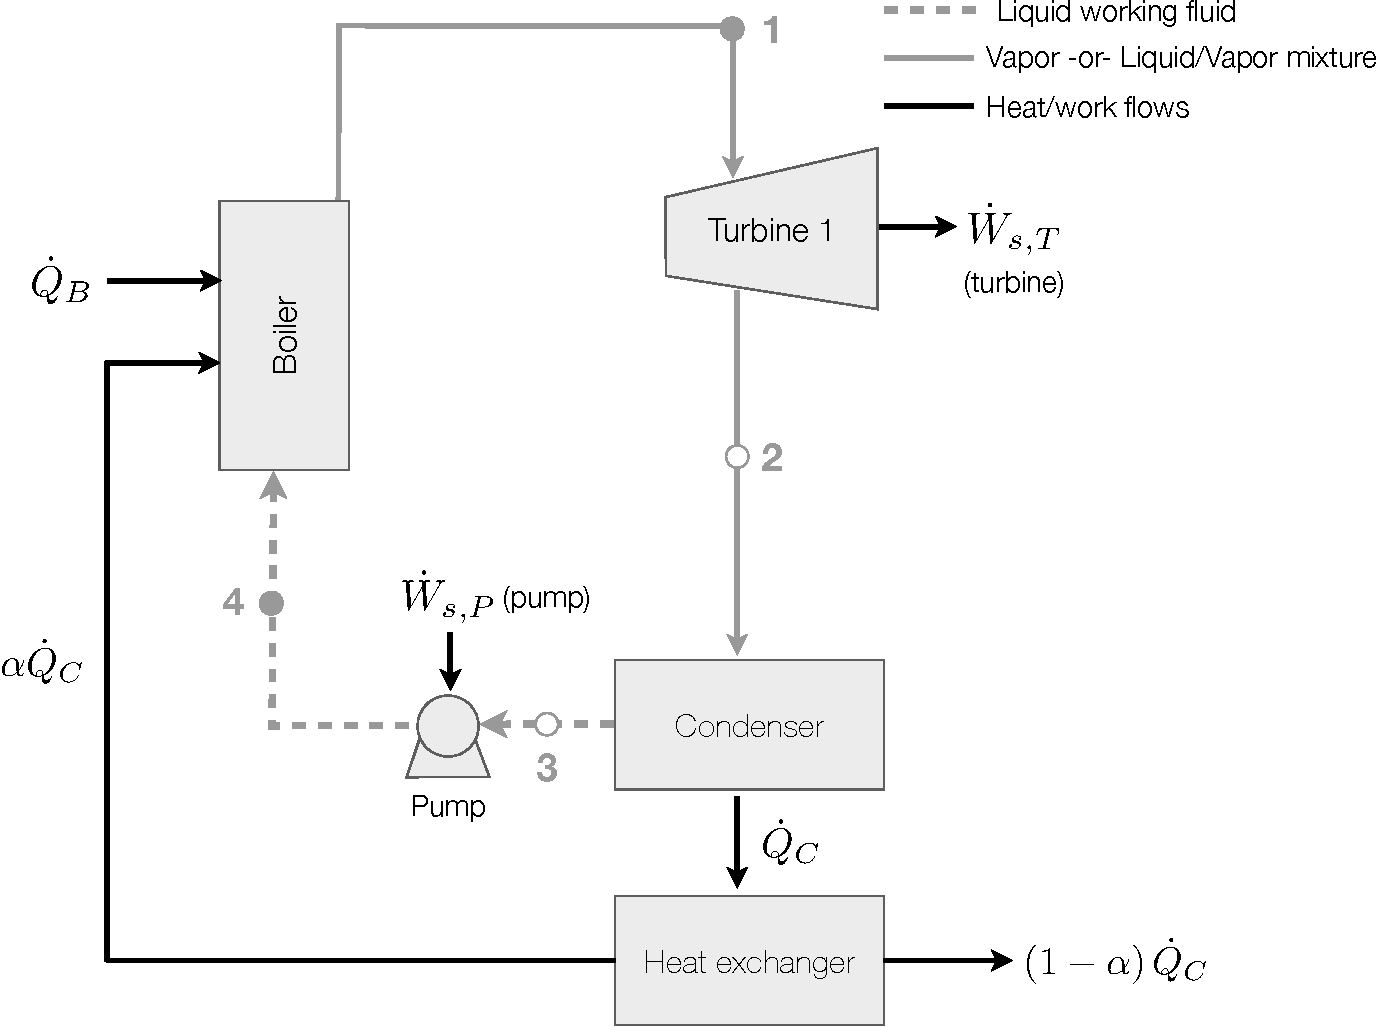
\includegraphics[width=0.72\textwidth]{./figs/Fig-Mod-Rankine-ENGRI-1120-F22.pdf}
    \caption{Schematic of the unit operations of a modified organic Rankine cycle in which a fraction of the heat from the condenser is recycled to the boiler through a heat exchanger.}\label{fig-rankine-cycle}
    \end{figure*}
    
    \item{(30 pt)~The Organic Rankine Cycle (ORC) is an \textit{open} four step thermodynamic process used to generate power that uses organic compounds as 
    working fluids (Fig. \ref{fig-rankine-cycle}). In the cycle, path $\mathcal{P}_{ij}$ connects operating point $\mathcal{O}_{i}$ to $\mathcal{O}_{j}$:
    \begin{itemize}
      \item[$\mathcal{P}_{41}$]{$\left(4~\rightarrow~1\right)$: \textit{isobaric} heating in a boiler from operating point $\mathcal{O}_{4}$ to $\mathcal{O}_{1}$}
      \item[$\mathcal{P}_{12}$]{$\left(1~\rightarrow~2\right)$: \textit{adiabatic} expansion in a turbine from operating point $\mathcal{O}_{1}$ to $\mathcal{O}_{2}$}
      \item[$\mathcal{P}_{23}$]{$\left(2~\rightarrow~3\right)$: \textit{isobaric} cooling in a condenser from operating point $\mathcal{O}_{2}$ to $\mathcal{O}_{3}$}
      \item[$\mathcal{P}_{34}$]{$\left(3~\rightarrow~4\right)$: \textit{adiabatic} compression in a pump from operating point $\mathcal{O}_{3}$ to $\mathcal{O}_{4}$}
    \end{itemize}

    \textbf{Nomenclature}: $\dot{W}_{s,T}$ denotes the rate of turbine shaft work (units: kJ s$^{-1}$); 
    $\dot{W}_{s,P}$ denotes the rate of pump shaft work (units: kJ s$^{-1}$); 
    $\dot{Q}_{B}$ denotes the rate of heat input/output to/from the boiler (units: kJ s$^{-1}$);
    $\dot{Q}_{C}$ denotes the rate of heat input/output to/from the condenser (units: kJ s$^{-1}$)
    
    \textbf{Assume}: (i) the cycle operates at steady-state; (ii) the working fluid (HFC-134A) has a mass flow rate of $\dot{m}$ = 2.25 kg s$^{-1}$;
    (iii) \textit{neglect} the enthalpy and temperature change from the pump (assume T$_{3}\simeq$~T$_{4}$ and H$_{3}\simeq$~H$_{4}$);
    (iv) neglect changes in the kinetic and potential energy in the system and streams; (v) the turbine efficiency $\eta_{T}$ = 85\%.
    
    \begin{itemize}
      \item[a)]{(12 pt)~Compute the missing state values in Table \ref{tbl-rankine-simple-state}.}
      \item[b)]{(12 pt)~Compute the missing values in Table \ref{tbl-rankine-simple-work} without heat recycle ($\alpha$ = 0).}
      \item[c)]{(3 pt)~Compute the ideal organic Rankine cycle efficiency: $\eta$ = $-\dot{W}_{net}$/$\dot{Q}_{B}$ if there is no heat recycle ($\alpha$ = 0).}
      \item[d)]{(3 pt)~Compute the ideal organic Rankine cycle efficiency if $\alpha$ = 0.33. Does the efficiency increase, decrease or stay the same when compared with c)?}
    \end{itemize}
    
    \clearpage
    
    \begin{table}[!ht]
      \centering
      \caption{State table for the ideal Rankine cycle problem with heat recycle.}\label{tbl-rankine-simple-state}
    
      \renewcommand{\arraystretch}{2.0}
      \setlength{\tabcolsep}{14pt}
      \begin{tabular}{c|c|c|c|c|c}\toprule
      $\mathcal{O}$ & T ($^{\mathrm{o}}$C) & P (MPa/kPa) & H (kJ kg$^{-1}$) & S (kJ kg$^{-1}$ K$^{-1}$) & Quality $\theta$ \\ \bottomrule
      $\mathcal{O}_{1}$ & 80.0 & 2.0 MPa & & 1.75 & 1.0 \\ \hline
      $\mathcal{O}_{2}$ &  & 29.41 kPa &  & 1.75 &  \\ \hline
      $\mathcal{O}_{3}$ & & & & & \\ \hline
      $\mathcal{O}_{4}$ & & & & 0.7428 & 0.0 \\ \bottomrule
      \end{tabular}
    \end{table}
    
    \clearpage
    
    \begin{table}[!ht]
      \centering
      \caption{Heat and work table for the Rankine cycle problem with heat recycle ($\alpha$ = 0).}\label{tbl-rankine-simple-work}
    
      \renewcommand{\arraystretch}{2.0}
      \setlength{\tabcolsep}{14pt}
      \begin{tabular}{c|c|c|c}\toprule
      Path & $\dot{Q}$ (kW) & (ideal)~$\dot{W}_{s}$ (kW) & (actual)~$\dot{W}^{*}_{s}$ (kW)\\ \bottomrule
      $\mathcal{P}_{12}$ & 0 & &  \\\hline
      $\mathcal{P}_{23}$ &  & 0 & 0 \\\hline
      $\mathcal{P}_{34}$ & N/A & N/A & N/A \\\hline
      $\mathcal{P}_{41}$ &  & 0 & 0 \\\bottomrule
      Cycle & & & N/A \\\bottomrule
      \end{tabular}
    \end{table}
      
    \clearpage
    }    
% ================================ %

% Question 3 ===================== %
\clearpage
\begin{figure*}[h!]\centering
  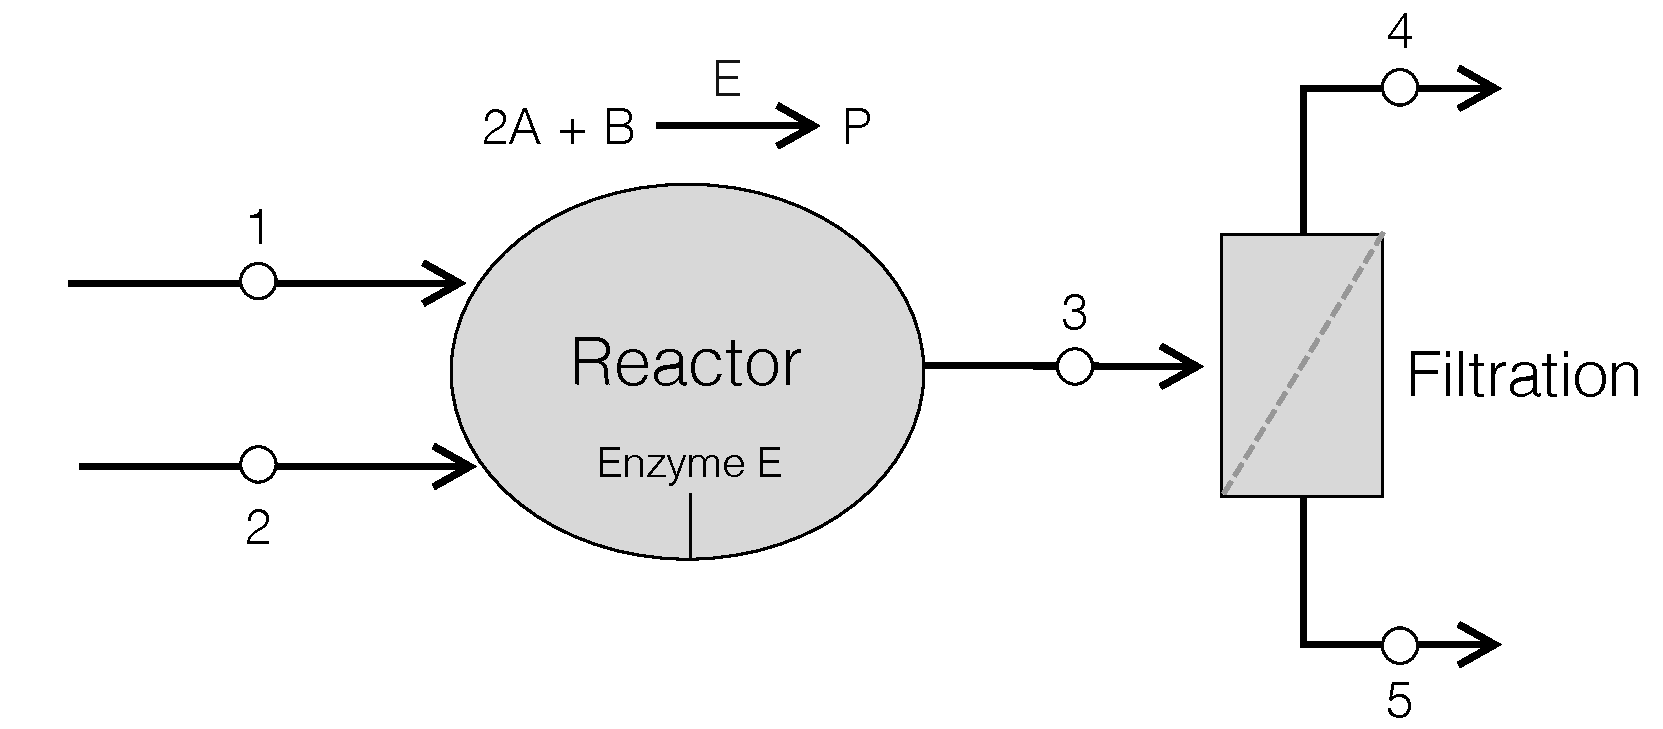
\includegraphics[width=0.80\textwidth]{./figs/Fig-Schematic-Reactor-Problem.pdf}
  \caption{Starting material(s) $A$ and $B$ are converted to product $P$ by enzyme $E$ in a well-mixed reactor with volume $V$. 
  The reactor is well insulated. 
  The output from the reactor is fed into a filtration unit that separates reactants and products.}\label{fig-reactor-splitter}
  \end{figure*}

    \item{(20 pt) Consider the reaction/separation process shown in Fig. \ref{fig-reactor-splitter}.
    In a well-mixed and well-insulated reactor, starting material(s) $A$ and $B$ are converted to the product $P$ by enzyme $E$.
    The enzyme $E$ is immobilized in the reactor (does not flow out) and is stable. Downstream of the reactor,
    a filtration device separates unreacted starting material(s) $A$ and $B$ from product $P$.
   
    \textbf{Assume}: (i) the reactor and filtration units operate at steady-state;
    (ii) let species $(A,B,P)$ have indexes $(1,2,3)$;
    (iii) there is no product in the input streams

    \begin{itemize}
        \item[a)]{~(16 pt)~Compute the missing values in Table \ref{tbl-reactor-filter} if the open extent of reaction $\dot{\epsilon}_{1}$ was measured to be 26.8 mmol min$^{-1}$.}
        \item[b)]{~(2 pt)~Derive an expression for the fractional conversion of species $i$, denoted by $f_{i}\geq{0}$ for the reactor configuration shown in Fig. \ref{fig-reactor-splitter}}. 
        \item[c)]{~(2 pt)~Using the expression from b), compute the fractional conversion for species $A$ and $B$.}

    \end{itemize}
    }


    \clearpage
    
    \begin{table}[!ht]
      \centering
      \caption{State table for the reaction/filtration problem; $\dot{n}_{s,T}$ denotes the total mole flow rate in stream $s$, 
      $x_{s,1}$ denotes the mole fraction of component 1 (A) in stream $s$, 
      $x_{s,2}$ denotes the mole fraction of component 2 (B) in stream $s$, and
      $x_{s,3}$ denotes the mole fraction of component 3 (P) in stream $s$.}\label{tbl-reactor-filter}
    
      \renewcommand{\arraystretch}{2.0}
      \setlength{\tabcolsep}{14pt}
      \begin{tabular}{c|c|c|c|c}\toprule
      Stream $i$ & $\dot{n}_{s,T}$ (mmol/min) & $x_{s,1}$ & $x_{s,2}$ & $x_{s,3}$ \\ \bottomrule
      1 & 95 & 1.0 & 0.0 & 0.0 \\ \hline
      2 & 45 & 0.11 & 0.89 & 0.0   \\ \hline
      3 & & & &   \\ \hline
      4 & & & & \\ \hline
      5 & 59.54 & 0.77 & 0.22 & 0.01 \\ \bottomrule
      \end{tabular}
    \end{table}
% ================================ %


% Question 4 ===================== %
% \clearpage
% \include{Q1_v1}
% ================================ %

% Extra -
\clearpage

\end{enumerate}

\end{document}
